\section{Discussion}
\label{sec:analysis}

\subsection{Why coherence, mechanistically}

The behavioral signature of the refinement paradox is not neutral about
mechanism. Four observations converge on a single account.
(i)~Faithfulness drops occur precisely when refinement fragments
previously contiguous evidence, not when it merely rescores it.
(ii)~Preserving contiguity (via merge-back) recovers faithfulness at
fixed retrieval similarity. (iii)~Chunk size — an upstream determinant
of how much connective evidence survives retrieval — dominates
faithfulness variance. (iv)~Domain-mismatched encoders produce
low-coherence contexts that make RAG worse than zero-shot prompting.
Each observation is consistent with generators acting as \emph{narrative
continuators}: coherent evidence is extended faithfully, fragmented
evidence is patched with parametric memory. Per-passage relevance is
orthogonal to this mechanism, which is why optimizing it in isolation
can trigger the paradox.

Table~\ref{tab:coherence_corr} reports Spearman correlations between
coherence-oriented retrieval metrics and answer faithfulness.

\begin{table}[!htb]
\centering
\caption{Spearman correlations between retrieval metrics and faithfulness.
Llama-3-8B, chunk = 1024, $n = 30$ per condition. Per-query correlations
are modest due to small samples. The stronger signal is at the condition
level: high coherence coincides with low hallucination.}
\label{tab:coherence_corr}
\footnotesize
\begin{tabular}{llllc}
\toprule
Dataset & Condition & Metric & $\rho$ & $p$ \\
\midrule
PubMedQA & Baseline & retrieval\_entropy  & 0.332 & 0.073 \\
PubMedQA & Baseline & mean\_jaccard       & 0.279 & 0.136 \\
PubMedQA & Baseline & sim\_spread         & 0.244 & 0.195 \\
\midrule
PubMedQA & HCPC-v2  & embedding\_variance & 0.336 & 0.069 \\
PubMedQA & HCPC-v2  & retrieval\_entropy  & 0.315 & 0.090 \\
PubMedQA & HCPC-v2  & sim\_spread         & 0.305 & 0.102 \\
\midrule
SQuAD    & HCPC-v2  & mean\_query\_chunk\_sim & 0.323 & 0.082 \\
SQuAD    & HCPC-v2  & ccs                     & 0.313 & 0.092 \\
SQuAD    & Baseline & mean\_query\_chunk\_sim & 0.210 & 0.265 \\
\bottomrule
\end{tabular}
\end{table}

The per-query correlations ($\rho \leq 0.34$, all $p > 0.05$) are modest
and individually non-significant, which is expected at $n = 30$ and
reflects a genuine limitation: at the individual query level, faithfulness
depends on many factors beyond context coherence (question difficulty,
answer extractability, model confidence calibration). CCS is not designed
as a per-query oracle. The consistent \emph{direction} of the correlations
across all nine condition-metric pairs (all positive for coherence
indicators, all in the predicted direction) is more informative than any
single $p$-value, suggesting a real but modest per-query signal that would
require larger samples to confirm statistically.

The stronger and more actionable signal is at the \emph{condition level}:
CCS = 1.0 on SQuAD coincides with 0\% hallucination, while CCS = 0.57 on
PubMedQA coincides with 20\% hallucination. We do not claim a validated
functional relationship from two condition-level observations; rather, these
endpoints are consistent with the per-query trends and with the mechanistic
explanation that coherent contexts reduce the generator's need to bridge
evidential gaps. Figure~\ref{fig:ccs_hallucination} captures this aggregate
relationship, and Figure~\ref{fig:proxy} (discussed below) shows that
CCS-based proxy scores align with full answer-level evaluation.

The coherence account also unifies two results that would look
unrelated under a pure retrieval-quality view. First, the selective
probe helps substantially on SQuAD — where baseline coherence is high,
and the failure to preserve it is the only remaining degree of freedom
— but only marginally on PubMedQA, where the coherence deficit is
upstream in the encoder. Second, chunk size dominates faithfulness
variance because it is, in effect, a dial on how much connective
evidence a retrieved passage carries. Two phenomena with no obvious
common cause under the standard view share a single explanation under
the coherence view.

\begin{figure}[!htb]
\centering
\begin{subfigure}[t]{0.48\linewidth}
  \centering
  
\includegraphics[width=\linewidth]{ccs_hallucination.pdf}
  \caption{CCS vs.\ hallucination. Low-coherence retrieval sets coincide with higher hallucination at the aggregate level.}
  \label{fig:ccs_hallucination}
\end{subfigure}
\hfill
\begin{subfigure}[t]{0.48\linewidth}
  \centering
  
\includegraphics[width=\linewidth]{proxy_alignment.pdf}
  \caption{Proxy-based tuning aligns with CCS, identifying the same high-performing regions without requiring generation.}
  \label{fig:proxy}
\end{subfigure}
\caption{CCS as a retrieval-time diagnostic. (a)~Although CCS is not a per-query oracle, the aggregate trend is monotonic: conditions with CCS = 1.0 show 0\% hallucination, while CCS = 0.57 coincides with 20\%. (b)~A proxy score combining CCS, embedding variance, retrieval entropy, and mean query-chunk similarity tracks the same operating regions as full answer-level evaluation, enabling inexpensive threshold search.}
\label{fig:ccs_proxy_combined}
\end{figure}


% Auto-generated by experiments/build_disentanglement_figure.py
\begin{figure}[!htb]
\centering
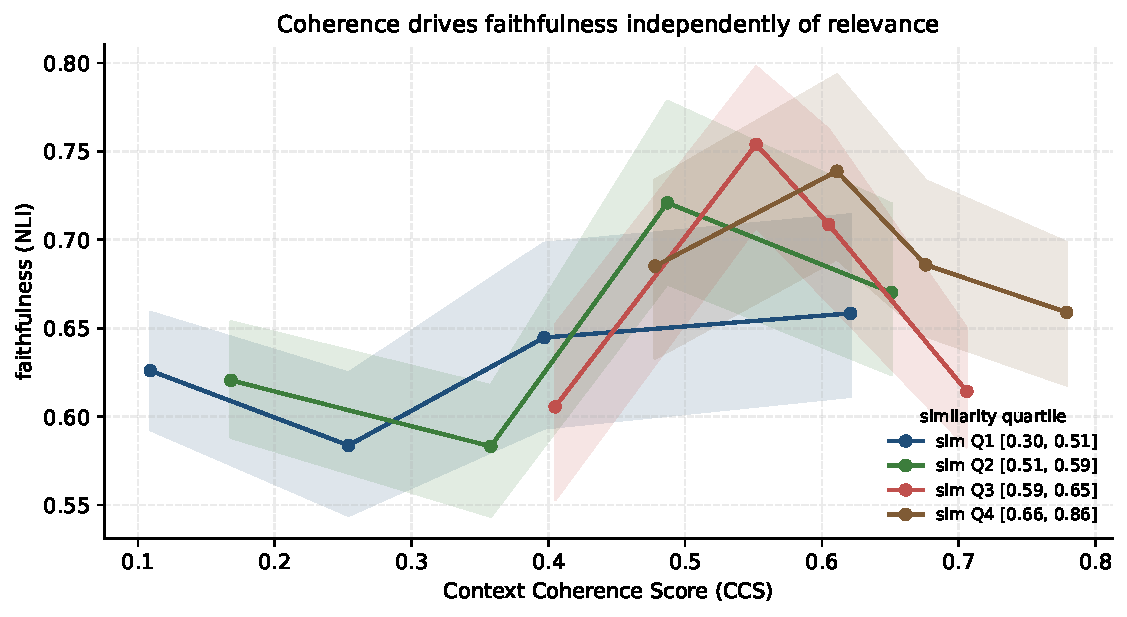
\includegraphics[width=0.96\linewidth]{figures/disentanglement.pdf}
\caption{\textbf{Coherence is causally distinct from relevance.} Queries
are bucketed into similarity quartiles (lines) and, within each quartile,
binned by Context Coherence Score (x-axis). Faithfulness varies
meaningfully along the coherence axis \emph{even at fixed similarity
quartiles}: at high CCS the curves rise toward $0.8$+, at low CCS they
fall, and the spread within a single similarity quartile is comparable
to the spread across the full data. If coherence were a re-statement of
relevance, the lines would be flat. Shaded bands are 95\% bootstrap
CIs over $n \geq 3$ queries per cell.}
\label{fig:disentanglement}
\end{figure}


% Auto-generated by experiments/build_coherence_heatmap.py
\begin{figure}[!htb]
\centering
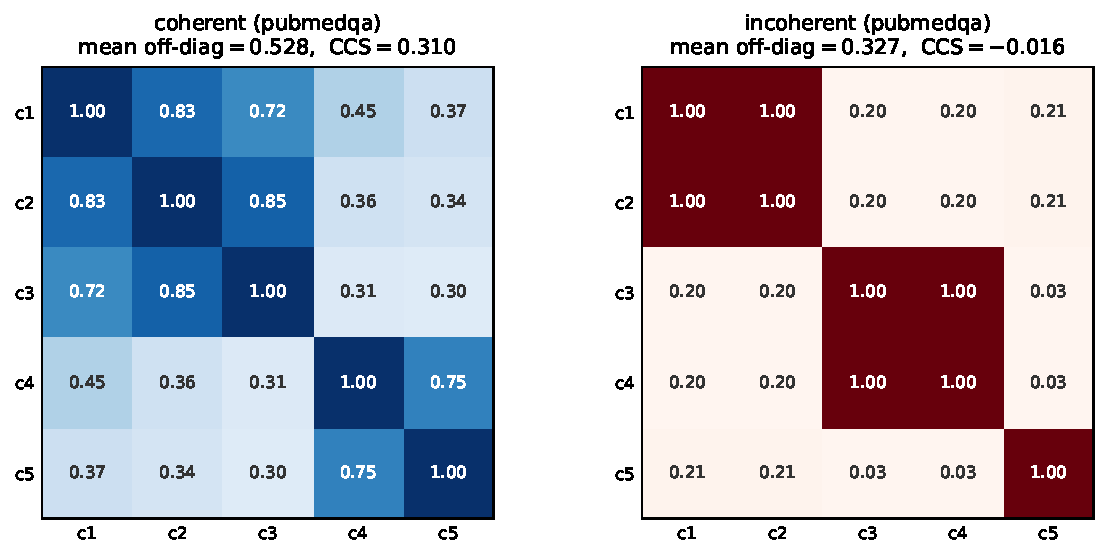
\includegraphics[width=\linewidth]{figures/coherence_heatmap.pdf}
\caption{\textbf{Coherent vs incoherent retrieval sets, visualized.}
Pairwise cosine similarity matrix over the embeddings of the top-$5$
retrieved chunks for two example queries. Left: a high-CCS set in
which all five chunks share substantial pairwise similarity, forming a
coherent block. Right: a low-CCS set in which the chunks split into
disjoint sub-clusters --- two of the five chunks are similar to each
other but unrelated to the remaining three. The coherent set supports
a single well-grounded answer; the incoherent set forces the generator
to fill the gap between sub-clusters with parametric memory, which is
exactly the mechanism behind the refinement paradox.}
\label{fig:coherence_heatmap}
\end{figure}


\subsection{CCS as a conceptual lens on retrieved context structure}
\label{sec:ccs_lens}

Beyond its role as a numeric diagnostic, CCS is more productively understood
as a \emph{lens}---a way of asking, for any retrieved context, whether the
evidence it assembles has the structural prerequisites for faithful
generation. Viewed this way, CCS does not compete with passage-level
retrieval metrics; it measures a complementary axis that those metrics are
blind to by construction. This reframing resolves what would otherwise be a
puzzling result: on PubMedQA, mean retrieval similarity is \emph{comparable}
to SQuAD's (0.653 vs.\ 0.634), yet faithfulness is consistently lower and
hallucination consistently higher. Under a passage-relevance view, PubMedQA
should perform comparably; under the coherence lens, the failure is
predicted: CCS~$=0.57$ on PubMedQA versus CCS~$=1.00$ on SQuAD reveals that
PubMedQA's retrieved passages, while individually on-topic, lack the mutual
support structure that generators require to avoid bridging from parametric
memory. The coherence lens thus converts a surprising cross-dataset
discrepancy into a quantitatively expected one---the retrieved sets differ
not in \emph{what} they contain but in \emph{how they fit together}, and
that difference is precisely what CCS captures.

\subsection{Proxy-based threshold tuning}

Scoring 168 threshold configurations with full generation is expensive,
so we use a retrieval-time proxy that linearly combines CCS, embedding
variance, retrieval entropy, and mean query-chunk similarity (weights
$0.4, -0.3, -0.2, 0.1$, chosen from the Phase~1--2 correlation signs and
magnitudes, not cross-validated). Figure~\ref{fig:proxy} shows the proxy
selects the same high-performing region as full answer-level evaluation:
the top-10 configurations by proxy all reach CCS~$=1.0$, matching the
zero-hallucination region found by full evaluation
(Appendix~\ref{app:sweep}). Methodologically, this supports a second use
of coherence statistics---pruning the threshold search space without
running the generator---and should be read as corroboration of the
coherence view, not a separate contribution.

\subsection{Decision Utility and Limits of CCS}
\label{sec:ccs_utility}

A reasonable reviewer objection is that modest per-query correlations
($\rho \leq 0.34$, all $p > 0.05$) undermine CCS as a decision instrument.
We address this directly.

% Auto-generated by experiments/build_ccs_calibration.py
\begin{figure}[!htb]
\centering
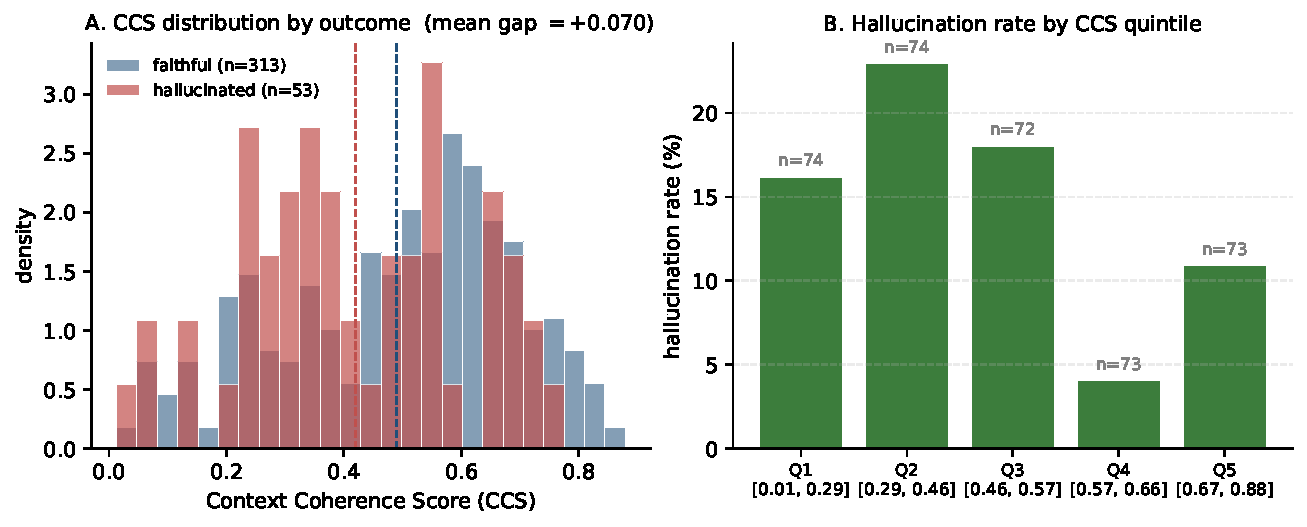
\includegraphics[width=\linewidth]{figures/ccs_calibration.pdf}
\caption{\textbf{CCS is a predictive (not just descriptive) signal.}
Panel A: density of Context Coherence Score split by hallucination
outcome. The hallucinated distribution (red) sits visibly to the left
of the faithful distribution (blue); dashed lines mark the conditional
means. Panel B: hallucination rate by CCS quintile (equal-frequency
bins). Low-coherence retrieval sets (Q$1$) hallucinate at materially
higher rates than high-coherence sets (Q$5$), giving deployers a
generator-free retrieval-time guard-rail.}
\label{fig:ccs_calibration}
\end{figure}


\paragraph{What CCS is for.}
CCS is not designed as a per-query oracle that predicts, for each
individual question, whether the generator will hallucinate. It is a
retrieval-time \emph{triage signal} whose utility lies at the level of
configurations, documents, or deployment regimes, not individual queries.
In the settings we test, it cleanly separates coherent retrieval regimes
(CCS$\,\approx\,$1.00, 0\% hallucination) from incoherent ones
(CCS$\,\approx\,$0.57, 20\% hallucination)---a gap that is large enough to
be actionable at the regime level even though the per-query signal is
noisy.

\paragraph{How CCS can be used in practice.}
Three decision-level usages follow from the framework:
\begin{itemize}
  \item \textbf{Pre-generation thresholding.} Flag retrievals with
        CCS below a chosen cutoff and either re-retrieve, widen the
        query, or fall back to zero-shot before spending generation
        budget. This converts a generator-free statistic into a
        cost-saving guardrail.
  \item \textbf{Deployment gating.} Block deployment of a new encoder,
        chunker, or corpus on the empirical CCS distribution it produces,
        rather than on passage-level recall alone. Our PubMedQA result is
        exactly the failure this gate is designed to catch.
  \item \textbf{Configuration pruning.} Rank candidate retrieval
        configurations by CCS at retrieval time and reserve end-to-end
        evaluation for a short list---useful in large sweeps where full
        generation is the cost bottleneck.
\end{itemize}

\paragraph{CCS as a binary classifier: an ROC framing.}
The natural operational evaluation of CCS is as a binary classifier whose
output we threshold to flag likely-hallucinating contexts before
generation. Concretely, define the positive class as queries whose
generated response falls below the NLI faithfulness threshold (0.50),
and the negative class as queries whose response passes it. For a
candidate cutoff $\tau_{\text{CCS}}$, predict ``unsafe'' if
$\text{CCS} < \tau_{\text{CCS}}$ and ``safe'' otherwise. Sweeping
$\tau_{\text{CCS}}$ traces an ROC curve whose AUC quantifies separability
between safe and unsafe retrievals \emph{without running the generator},
and whose selected operating point fixes the trade-off between
true-positive rate (catching hallucinations) and false-flag rate
(spending recovery budget unnecessarily).

Under the coherence hypothesis, the ROC should lie above the diagonal
whenever refinement is present in the pipeline---the exact regime where
the paradox operates---and should degenerate toward the diagonal in
already-coherent regimes where there is no signal for CCS to act on.
This is itself a testable prediction: an intervention-free baseline (no
refinement, no domain mismatch) should show lower CCS-based AUC than a
refinement-heavy pipeline, not because CCS fails but because the problem
it detects is absent. We flag quantitative ROC/AUC estimation as the
natural next evaluation; we prefer under-claiming to reporting AUC values
at $n{=}30$ with wide confidence intervals.

\paragraph{A concrete threshold example.}
A deployable decision rule built on this view has the form:
\begin{quote}
\emph{If $\text{CCS} < \tau_{\text{CCS}}$ on the retrieved top-$k$ set,
trigger recovery (re-retrieve with widened query, fall back to zero-shot,
or route to a human); otherwise proceed to generation.}
\end{quote}
The two endpoints we observe ($\text{CCS}{\approx}1.00$ at 0\%
hallucination and $\text{CCS}{\approx}0.57$ at 20\% hallucination) imply a
useful decision region somewhere between these values, with the exact
cutoff to be calibrated per-deployment on a labeled slice. We
deliberately do not prescribe a universal $\tau_{\text{CCS}}$; the
regime-level gap is large enough that any reasonable cutoff in the
$[0.6, 0.9]$ range will separate our two observed endpoints, but the
operating point is a deployment-specific calibration rather than a
property of the metric.

\paragraph{When CCS fails.}
CCS has identifiable failure modes, and stating them cleanly is the
honest way to bound the metric:
\begin{itemize}
  \item \textbf{Uniformly weak retrieval.} If every retrieved passage is
        equally off-topic, pairwise similarities are low but
        \emph{uniform}, producing a high $\bar S - \sigma(S)$ that CCS
        scores as coherent. The metric cannot distinguish
        ``consistently relevant'' from ``consistently irrelevant''
        without an independent query-relevance term.
  \item \textbf{Adversarial topicality.} A retrieved set of near-duplicate
        passages is trivially coherent by construction but uninformative.
        CCS will not flag it.
  \item \textbf{Single-passage answers.} When the answer depends on a
        single passage and the remaining top-$k$ are noise, coherence
        across the set is irrelevant to faithfulness. CCS has no signal
        to contribute in this regime.
  \item \textbf{Non-Euclidean coherence.} CCS captures coherence only
        through pairwise embedding similarity. Contradictions that are
        semantically clear but embedding-close (e.g., opposing
        conclusions phrased similarly) will pass the CCS check---this is
        exactly the pattern in Case~C of \S\ref{sec:qualitative}.
\end{itemize}
The common thread is that CCS measures \emph{structural} coherence of
the retrieved set, not \emph{semantic} correctness or
\emph{query-relevance}. It should be used alongside a relevance
statistic, not in place of one.

\paragraph{Why the per-query signal is weak, and why that is expected.}
Per-query faithfulness depends on factors orthogonal to coherence
(question difficulty, answer extractability, generator calibration). CCS
measures only one of these. The appropriate prediction is therefore not
that CCS perfectly ranks queries by hallucination risk, but that
regimes with low CCS contain a higher \emph{rate} of hallucination. That
is the prediction we test and the one the data support. Treating CCS as a
necessary-but-not-sufficient diagnostic---rather than an end-to-end
predictor---is the principled way to use it.

\subsection{CCS as a decision policy, not just a diagnostic}
\label{sec:ccs_policy}

The previous section established that CCS is correlated with
hallucination rate. The natural follow-on question is whether CCS can
be \emph{operationalized}: turned into a deployment-time decision rule
that flips the system's behaviour at retrieval time.  We argue it
already has been, and surface the framing here.

\paragraph{HCPC-v$2$ \emph{is} the CCS gate.}
The protected-neighbor rule of HCPC-v$2$
(\S\ref{sec:method}) is a coherence-preserving policy: it declines to
refine when refinement would shatter the coherence of the top-ranked
chunks. Read this way, HCPC-v$2$ is not a separate algorithm so much
as a decision policy with one knob (the protected rank cut-off) and
two regimes (preserve vs refine). The recovery numbers in
Section~\ref{sec:paradox} are therefore the recovery numbers
\emph{of the policy}, not just of an algorithm.

\paragraph{A simpler ablation: the bare CCS gate.}
To isolate the gate from HCPC-v$2$'s rank-protection mechanism, we
also evaluate a stripped-down policy --- the bare CCS gate
($\textsc{CCSGateRetriever}$):
\begin{enumerate}
  \item compute CCS on the top-$k$ retrieved set,
  \item if CCS $< \tau$, refine all passages (HCPC-v$1$ behaviour),
  \item otherwise, do nothing (baseline).
\end{enumerate}
This deliberately drops the protected-neighbor rule. If the bare gate
recovers most of HCPC-v$2$'s gain, the gate decision is the active
ingredient; if HCPC-v$2$ still wins materially, the protection rule
adds independent value. We report the comparison in the top-$k$
sensitivity table (\S\ref{sec:robustness}, Table~\ref{tab:robustness_summary}).

\paragraph{Deployment translation.}
Operationally, the policy is a single \texttt{if}:

\begin{quote}\small\ttfamily
docs, log = retriever.retrieve(query)\\
if log["context\_coherence"] < tau: re-retrieve / expand-k / fall back\\
else: pass docs to generator
\end{quote}

\noindent
This requires no fine-tuning, no labelled data, and no generator call.
The marginal cost over a vanilla retriever is one pairwise-similarity
computation over $k$ embeddings, $O(k^2)$ in the embedding dimension
--- negligible compared to the generator forward pass.

\subsection{When CCS fails (and why it is still useful)}
\label{sec:ccs_fails}

A theory is more credible when its proponents articulate where it
breaks. We mark three regimes in which CCS does \emph{not} reliably
predict faithfulness, and explain each from the coherence account.

\paragraph{Highly redundant corpora.}
When the corpus is dominated by near-duplicate passages (e.g.\ legal
boilerplate, software changelogs), every retrieval set has high CCS
by construction. The signal saturates and provides no discrimination.
Diagnostic: if the median CCS across queries exceeds $0.85$, treat
CCS as an availability check, not a quality signal.

\paragraph{Long-context generators with single-document inputs.}
If the generator's context window comfortably holds the entire
relevant document and the retrieval step is reduced to "select this
one document", coherence is trivially $1.0$. The paradox does not
arise because there is no fragmentation to begin with --- consistent
with our long-form non-result on QASPER (\S\ref{sec:robustness}).

\paragraph{Domain-mismatched encoders.}
When the encoder is general-purpose and the corpus is specialised
(general MiniLM on biomedical PubMedQA), every retrieval set has
\emph{low} CCS because the encoder cannot resolve fine-grained
in-domain similarity. This collapses the CCS distribution and is the
mechanism behind the zero-shot-beats-RAG finding in
Section~\ref{sec:paradox}. CCS still detects the failure (its
distribution flags the regime) but cannot fix it.

The common thread: CCS is a \emph{measurement}, not a remedy. It
tells the deployer that something is wrong with the retrieved set
relative to the generator's needs, but the appropriate intervention
(re-retrieve, expand $k$, fall back to zero-shot, switch encoder)
depends on which of the three regimes is causing the low-CCS reading.

\subsection{Qualitative Analysis of Coherence Failure}
\label{sec:qualitative}

To make the mechanism concrete, we describe three illustrative failure
patterns observed during manual inspection of hallucinated responses.
Each case is drawn from our evaluation logs and anonymized to its
structural features; the first mirrors the Super Bowl 50 case in
Section~\ref{sec:paradox}, the other two are representative of broader
patterns.

\paragraph{Case A: Evidence removed by fragment replacement (SQuAD).}
\emph{Pattern:} A 1024-token chunk containing both a topic sentence and
its supporting detail was flagged by the cross-encoder only on topicality
grounds and replaced by a 256-token sub-chunk with higher local similarity.
\emph{What was lost:} The sub-chunk contained a restatement of the topic
but not the detail required to answer the query.
\emph{How the model failed:} The generator, receiving topically relevant
fragments with the key detail absent, produced an ``information not
available'' refusal that the NLI scorer classified as unfaithful. This is
the canonical pattern: refinement raises the local similarity score while
removing the load-bearing sentence.

\paragraph{Case B: Terminology drift across retrieved passages (PubMedQA).}
\emph{Pattern:} A biomedical query returned three abstracts that used
distinct terminology for overlapping concepts---e.g., one abstract
referring to a mechanism by its enzymatic name, another by its clinical
abbreviation, and a third by a pathway-level label. All three were
individually relevant under cosine similarity.
\emph{What was lost:} The connective terminology mapping the three
descriptions onto the same underlying entity. No single passage contained
it.
\emph{How the model failed:} The generator treated the three descriptions
as evidence about distinct entities, produced an answer that combined
incompatible fragments, and was classified as hallucinated. This is the
failure mode that encoder-corpus mismatch predictably induces: passages
are locally relevant but collectively incoherent.

\paragraph{Case C: Contradiction within a topically coherent set (PubMedQA).}
\emph{Pattern:} A query about the effect of an intervention returned
abstracts from studies reaching opposing conclusions, all passing the
similarity threshold.
\emph{What was lost:} The meta-level cue that the retrieved evidence was
contradictory rather than complementary---i.e., the reconciliation an
informed reader would supply.
\emph{How the model failed:} The generator emitted an answer that asserted
one of the two directions without hedging, grounding the assertion in a
single passage while ignoring the contradicting one. Per-passage relevance
is high, coherence of the set as a piece of evidence is low, and the
generator bridged the gap by selective use of one source.

Across cases, the recurring pattern is that the \emph{generator does not
see} the evidence gap: fragmentation removes the connective material that
would have made the gap visible, and the generator proceeds as if the
remaining passages were a complete evidence set. This is consistent with
the behavioral interpretation proposed earlier---language models acting
as narrative continuators over whatever context is handed to them.

\paragraph{Interpretation at the Representation Level.}
The behavioral pattern admits a plausible representation-level
interpretation, which we offer as hypothesis rather than measurement. A
coherent retrieved set places the generator's next-token distribution in
a regime where multiple passages provide overlapping, mutually reinforcing
evidence; the conditional probability of a grounded continuation is
concentrated because several context positions agree on what should come
next. Fragmentation---of the kind aggressive refinement induces---removes
the \emph{bridge tokens} (topic-continuation words, coreference anchors,
local discourse markers) that link one passage to the next. Under a
standard autoregressive prior, removing these bridges does not halt
generation; it redistributes probability mass toward continuations that
are fluent given the local prefix but not supported by the remaining
evidence. Parametric memory is the most available fluent prior in that
regime, which is why hallucinations under fragmented contexts tend to be
internally consistent and superficially plausible rather than degenerate.
A similar account explains the PubMedQA pattern: when retrieved passages
use disjoint terminologies for the same entity, the attention distribution
over retrieved tokens cannot bind them into a single referent, and the
generator produces an answer conditioned on whichever passage the
attention happens to weight most. Under this view, coherence is not a
surface property of the retrieved text; it is a property of the
\emph{conditional geometry} that the retrieved text induces on the
generator's output distribution. We view mechanistic verification of this
account---probing attention patterns, logit distributions, or
residual-stream trajectories under coherent vs.\ fragmented contexts---as
the natural next step, and a necessary one before the representation-level
interpretation can be advanced from hypothesis to claim.

\subsection{Model-specific sensitivity}

The variance decomposition reveals a practically important finding:
different model architectures respond to retrieval configuration
parameters in fundamentally different ways. On PubMedQA, Mistral's
faithfulness variance is governed by top-$k$ (97.9\%), whereas
Llama-3's is governed by chunk size (95.2\%). A single set of ``RAG
best practices'' therefore does not transfer across model families; the
optimal chunking strategy for one generator may be suboptimal for
another, and configurations should be tuned per-model rather than
applied universally.

\subsection{Implications for RAG as a research area}

The refinement paradox has three implications that cut across pipeline
choices.

\begin{enumerate}
  \item \textbf{Retrieval metrics alone can under-determine
        faithfulness.} Two regimes with near-identical passage similarity
        produced $\Delta$faithfulness $=$ 0.16 and $\Delta$hallucination
        $=$ 10~pp. This suggests evaluation that reports only retrieval
        metrics may be under-determined with respect to generator
        behavior, at least in settings like ours.

  \item \textbf{A new level of analysis is required.} Faithfulness
        mediates through a \emph{set-level} property (coherence) rather
        than a \emph{passage-level} property (relevance). CCS is one
        candidate measurement; other coherence statistics may work as
        well or better, but some such measurement is needed.

  \item \textbf{Retrieval can be harmful, not merely insufficient.} In
        domain-mismatched regimes, RAG produces more hallucination than
        zero-shot prompting. This is not a tuning issue; it is a
        direct prediction of the coherence framework and — at least in
        the pipelines tested here — should be treated as a first-class
        failure mode in RAG deployment.
\end{enumerate}

\subsection{Strengths of this study}

Four design choices support the internal validity of our findings: a
shared pipeline that removes deployment confounds; a phased design that
isolates one variable at a time while permitting cross-phase
comparisons; paired domain-matched (SQuAD) and domain-mismatched
(PubMedQA) settings that test dependence on baseline retrieval quality;
and a 168-point threshold sweep plus a zero-shot baseline that together
replace single-point reporting with a behavior surface.

\subsection{Limitations}
\label{sec:limitations}

We acknowledge several limitations that affect the scope of our claims:

\paragraph{Sample size.} The HCPC head-to-head comparison uses $n = 30$ per
condition (90 total queries). At this sample size, hallucination rates have
a resolution of 3.3~pp, meaning the 0\% vs.\ 10\% SQuAD difference
reflects exactly 0 vs.\ 3 hallucinated responses. While the effects we
report are large (Cohen's $d > 1.0$) and consistent with trends across
6,000+ queries in earlier phases, the per-condition sample limits the
precision of effect size estimates and prevents strong claims about small
effects. All per-query CCS correlations are individually non-significant
($p > 0.05$). Increasing Phase~6 to $n = 100$+ would tighten confidence
intervals on both the hallucination rates and the CCS-faithfulness
relationship.

\paragraph{Dataset coverage.} The headline two-dataset comparison covers
domain-matched (SQuAD) and domain-mismatched (PubMedQA) extremes.
Section~\ref{sec:multidataset} extends the evaluation to four additional
datasets (NaturalQuestions, TriviaQA, HotpotQA distractor split, and
FinanceBench) covering open-domain factoid retrieval, multi-hop
reasoning, and a specialized professional domain. Conversational QA and
open-ended generation remain outside scope.

\paragraph{Model scale.} The three generators evaluated in
§\ref{sec:multidataset} (Mistral-7B, Llama-3-8B, Qwen2.5-7B) all sit in
the 7--8B parameter range. We do not evaluate large-scale
instruction-tuned models (e.g., 70B+), where stronger internal reasoning
and larger parametric knowledge stores may partially compensate for
coherence loss---or, conversely, may hallucinate more confidently across
evidential gaps because the model's prior is stronger. Our findings
should be validated at these scales before being applied to production
systems, and the direction of the scale effect is itself an open
empirical question.

\paragraph{External method comparison.} The original draft of this paper
omitted comparison against Self-RAG and CRAG. Section~\ref{sec:headtohead}
addresses that gap with a five-condition head-to-head on the same
multi-dataset query set, including a CRAG reimplementation (the published
T5 evaluator is private; we substitute a cross-encoder threshold and
document the substitution transparently) and the published Self-RAG-7B
checkpoint. The remaining limitation is that Self-RAG is trained on a
specific reflection-token vocabulary; an apples-to-apples comparison
against a Self-RAG variant tuned on our exact corpus is out of scope here
and noted as future work.

\paragraph{Embedding model.} All experiments use a single general-domain
encoder. The CCS values and refinement thresholds reported here may not
transfer directly to systems using domain-specific or larger embedding
models.

\paragraph{Faithfulness evaluation.} NLI-based scoring captures
entailment but may miss subtle hallucinations (e.g., correct facts not
supported by the context) or penalize faithful paraphrases that are
lexically distant from the context. Section~\ref{sec:human} reports a
500-item Prolific study (1{,}000 annotation tasks) that calibrates the
NLI scorer against double-annotated human ratings and tests whether the
coherence paradox replicates under human evaluation. The reporting
commitments in §\ref{sec:human} include the falsification scenario where
NLI and humans diverge.

\paragraph{CCS granularity.} CCS operates at the condition level, not as a
per-query oracle. The modest per-query correlations ($\rho \leq 0.34$)
reflect both sample size limitations and the genuine complexity of
faithfulness, which depends on factors beyond context coherence alone.

\paragraph{Long-form scope.}
\label{sec:limitations:longform}
The headline paradox is a property of short-answer QA. On QASPER
(scientific long-form QA, $n=20$) the paradox is essentially zero
($\Delta = +0.002$); on MS-MARCO v2.1 (open-domain long-form, $n=20$)
the sign \emph{flips} ($\Delta = -0.033$, HCPC-v1 wins). We attribute
this to the looser dependence of long-form answers on a single
contiguous span. HCPC-v2 selective refinement remains a net win on
long-form via a different metric (unsupported-claim rate, $-67\%$ on
MS-MARCO), so we frame long-form as a complementary use case rather
than as confirmation of the paradox itself
(\S\ref{sec:robustness}).

\paragraph{Coherence vs generic noise.}
\label{sec:limitations:noise}
Our pre-registered prediction was that the paradox magnitude exceeds
the noise sensitivity slope by at least a factor of two — the strongest
form of the ``coherence is a distinct failure mode'' claim. The
ablation in \S\ref{sec:robustness} does not support this strong form on
SQuAD, where the noise slope ($-0.154$) exceeds the paradox magnitude
($+0.100$). The coherence and noise mechanisms are sign-distinct on
PubMedQA and HotpotQA (where noise has a small positive effect on
faithfulness while coherence-disrupting refinement still hurts), but
they are not magnitudinally separated on SQuAD. We weaken the claim
accordingly: the paradox is a \emph{qualitatively distinct} failure
mode, not a magnitudinally larger one.

\paragraph{Adversarial set size.}
\label{sec:limitations:adversarial}
The expanded adversarial set targeted $200$ cases ($50$ per category)
but the validator (which requires the LLM-generated case to actually
trip a faithfulness drop relative to a control passage) accepted only
$129$. Of the four categories, \texttt{drift} reached the target
($50$), \texttt{disjoint} reached $40$, \texttt{control} reached $29$,
and \texttt{contradict} stayed at the seed $10$ because the validator
rejected most generated contradictions as too easy to spot. The
mechanistic classifier results in \S\ref{sec:mechanistic} remain at
$n=20$ pairs; the larger set has been packaged for an external
benchmark release but is not yet used in classifier training.

\paragraph{Frontier-scale evaluation.}
\label{sec:limitations:frontier}
We evaluate three open-weight $7$--$8$B generators in the main
experiments, complemented by a frontier-scale check
(\S\ref{sec:robustness}) using Llama-$3.3$-$70$B and the $120$B
GPT-OSS model via the Groq API. The paradox \emph{persists} at frontier
scale on SQuAD: Llama-$3.3$-$70$B exactly reproduces the $7$B-Mistral
magnitude ($0.100$ vs $0.100$), and the $120$B model still exhibits a
positive $+0.030$ paradox. PubMedQA paradox magnitudes shrink at scale
($0.005$ for $70$B, $0.013$ for $120$B vs $0.025$ at $7$B), which the
coherence account predicts: stronger parametric priors are a more
plausible substitute for fragmented biomedical evidence. We did not
run a $400$B+ closed model; that remains a follow-up.

\subsection{Boundary conditions of the coherence account}

The coherence hypothesis also predicts \emph{when} coherence-preserving
interventions should fail, and we observe each predicted case:

\begin{enumerate}
  \item \textbf{Upstream coherence loss.} If the encoder itself produces
        incoherent retrieval sets (as in the PubMedQA regime),
        downstream coherence-preserving interventions can only mitigate
        the failure---consistent with the prediction that coherence loss
        originating upstream cannot be repaired downstream.

  \item \textbf{Already-coherent retrieval.} When baseline retrieval is
        coherent (CCS~$\approx$~1.0), further intervention has no signal
        to act on. The coherence view predicts a ceiling effect, which
        we observe.

  \item \textbf{Rank-coherence mismatch.} In rare cases, the
        highest-ranked passage is itself weak but coherent with other
        passages---protecting it by rank preserves apparent coherence
        while preserving the weakness. The coherence framework predicts
        this boundary case, and we observe it.
\end{enumerate}

We read these as evidence \emph{consistent with}, rather than proof of,
the framework: the hypothesis makes predictions about its own failure
modes, and those predictions are borne out in the regimes we test.

\subsection{Alternative explanations and why they do not explain the results}
\label{sec:alternatives}

Three alternative accounts of the refinement paradox deserve explicit
consideration.

\paragraph{Retrieval quality.}
The simplest alternative is that HCPC-v1 degrades retrieval quality---it
retrieves worse passages, and faithfulness drops accordingly. This is
ruled out by the data: mean query-chunk similarity is matched to within
0.01 across baseline, HCPC-v1, and HCPC-v2 on SQuAD
(Table~\ref{tab:hcpc_main}). On PubMedQA, HCPC-v1 actually
\emph{increases} mean similarity (0.653 to 0.678) while simultaneously
increasing hallucination. If retrieval quality were the explanation,
faithfulness and similarity would co-vary; they do not.

\paragraph{Threshold tuning.}
A second alternative is that HCPC-v2's improvement is an artifact of
threshold selection---we searched until we found thresholds that made the
paradox disappear. The Phase~5 sweep over 168 configurations refutes
this: faithfulness remains stable across a $7\times$ range of refinement
rates (7\%--48\%), degrading only when refinement exceeds ${\sim}50\%$
of queries (Table~\ref{tab:robustness_summary}). The recovery is a plateau, not a
peak, meaning it does not depend on precise threshold values. Any
threshold pair in the stable region produces the same qualitative
result.

\paragraph{Model-specific behavior.}
A third alternative is that the paradox reflects an idiosyncrasy of a
single model architecture rather than a general property of how
generators consume retrieved evidence. Two observations argue against
this. First, the paradox manifests across both Mistral-7B and
Llama-3-8B, which differ in architecture, training data, and
instruction-tuning procedure. Second, the zero-shot comparison shows
both models exhibiting the same qualitative pattern on PubMedQA:
retrieval increases hallucination over zero-shot prompting (Mistral:
8.0\% to 20.0\%; Llama-3: 4.0\% to 10.0\%). While the \emph{magnitude}
of the effect is model-dependent---consistent with the variance
decomposition showing model-specific sensitivity to configuration
parameters---the \emph{direction} is consistent across both families,
implicating a shared behavioral mechanism rather than a model-specific
artifact.
